\chapter{Domande}

\section{Lullo, Leibniz e la storia del calcolo}

\qs{}{Che cos'è l'Ars Magna di Lullo?}

\paragraph{Risposta:} L'Ars Magna di Lullo è un'opera scritta da Raimondo Lullo, un filosofo, teologo e mistico catalano,
che trattava di un metodo per risolvere i problemi logici attraverso l'uso di diagrammi e figure.
In questo modo si potevano raggiungere verità in ogni campo del sapere.

\subsubsection{}

\qs{}{Quali sono le funzioni della combinatoria di Lullo?}

\paragraph{Risposta:} L'Ars Combinatoria di Lullo è un metodo inventivo
che permette di elaborare dimostrazioni allo scopo di convertire gli "infedeli" al cristianesimo\footnote{Sì, lo scopo era proprio quello.}.   

\subsubsection{}

\qs{}{Elencare almeno tre dei principi alla base della caratteristica universale di Leibniz.}

\paragraph{Risposta:}

\begin{itemize}
    \item [$\Rightarrow$] Le idee sono analizzabili;
    \item [$\Rightarrow$] L'analisi termina con le idee primitive;
    \item [$\Rightarrow$] Le idee possono essere rappresentate da simboli;
    \item [$\Rightarrow$] Le relazioni tra le idee possono essere rappresentate da simboli;
    \item [$\Rightarrow$] Le idee possono essere combinate, tramite opportune regole, per ottenere nuove idee.
\end{itemize}

\subsubsection{}

\qs{}{Elencare le principali caratteristiche della lingua universale.}

\paragraph{Risposta:}

\begin{itemize}
    \item [$\Rightarrow$] Segni che rappresentano direttamente le nozioni e le cose, non le parole;
    \item [$\Rightarrow$] Segni composti da figure geometiche e da pitture;
    \item [$\Rightarrow$] Direttamente collegata con l'enciclopedia;
    \item [$\Rightarrow$] Connessioni tra i caratteri corrispondono alle connessioni tra le cose;
    \item [$\Rightarrow$] I caratteri della lingua universale esprimono relazioni tra pensieri.
\end{itemize}

\subsubsection{}

\qs{}{Fare un esempio di proposizione dal frammento XX di Leibniz.}

\paragraph{Risposta:} Se $A \geq B$ e $B \geq C$, allora $A \geq C$.

\subsubsection{}

\qs{}{Qual è l'idea alla base di un approccio "pointless" alle nozioni geometriche e topologiche?}

\paragraph{Risposta:} L'idea alla base di un approccio "pointless" è quella che la classe
degli spazi aperti di uno spazio topologico costituisce un reticolo rispetto all'inclusione
per cui vale la proprietà di distributività.

\subsubsection{}

\qs{}{Che cosa è lo Entscheidungsproblem formulato da Hilbert e Ackermann nel 1928?}

\paragraph{Risposta:} L'Entscheidungs problem è un problema matematico che consiste nel determinare
un modo combinatorio finito per il quale combinazioni di simboli primitivi conducono a dimostrazioni.
In altre parole, trovare una procedura che consente di decidere la validità di una data
espressione logica con un numero finito di operazioni.

\section{Turing e la fisica del calcolo}

\qs{}{Perché Turing richiede che i simboli che possono essere scritti sul nastro 
di una macchina di Turing siano elementi di un insieme finito?}

\paragraph{Risposta:} Perché se l'insieme dei simboli fosse infinito, ci sarebbero un numero infinito di 
simboli molto simili tra loro, rendendo impossibile distinguerli.

\subsubsection{}

\qs{}{Perché Turing richiede che gli stati che possono essere assunti dall'unità
 di controllo di una macchina di Turing siano elementi di un insieme finito?}

\paragraph{Risposta:} Perché c'è un limite alla percezione delle caselle del nastro determinato dallo stato mentale.

\subsubsection{}

\qs{}{Che cosa stabilisce il procedimento diagonale di Cantor?}

\paragraph{Risposta:} Il procedimento diagonale di Cantor stabilisce che non esiste una corrispondenza biunivoca tra
l'insieme dei numeri naturali e l'insieme dei numeri reali. Serve a dimostrare il fatto che non tutte le funzioni 
siano calcolabili\footnote{E, per estensione, calcolabili da una macchina di Turing.}.

\subsubsection{}

\qs{}{Qual è la relazione tra una macchina di Turing generale e un automa finito?}

\paragraph{Risposta:} Un automa finito è una macchina di Turing generale con un nastro finito.

\subsubsection{}

\qs{}{Quali sono state le tappe fondamentali della formalizzazione degli automi finiti?}

\paragraph{Risposta:}

\begin{itemize}
    \item [$\Rightarrow$] Reti di neuroni di McCulloch e Pitts;
    \item [$\Rightarrow$] Eventi regolari di Kleene;
    \item [$\Rightarrow$] Lavoro di Rabin e Scott.
\end{itemize}

\subsubsection{}

\qs{}{Che cos'è il gioco della vita di Conway?}

\paragraph{Risposta:} Il gioco della vita di Conway è un automa cellulare bidimensionale (gioco a zero giocatori).
Il risultato di ogni generazione è determinato dallo stato della precedente secondo semplici regole.

\subsubsection{}

\qs{}{Qual è la relazione tra termodinamica e teoria dell'informazione?}

\paragraph{Risposta:} Von Neumann cercò di valutare il costo energetico minimo 
per un atto elementare di generazione di informazione ($kT \ln N$), ma Landauer
non riuscì a provarlo.

\subsubsection{}

\qs{}{Che cos'è il Principio di Landauer?}

\paragraph{Risposta:} Le operazioni logicamente irreversibili (cancellazione di bit) 
generano entropia pari alla quantità di informazione cancellata.

\subsubsection{}

\qs{}{Quali sono le difficoltà nell'applicazione della logica matematica classica alla formalizzazione di automi 
che descrivano sia i computer che il cervello umano?}

\paragraph{Risposta:} L'assiomatizzazione a scatole nere non è sufficiente per descrivere
il comportamento di un computer in relazione al comportamento del cervello umano.

\subsubsection{}

\qs{}{Quali sono, secondo Landauer, le operazioni che aumentano l'entropia nel processo di calcolo?}

\paragraph{Risposta:} Le operazioni che aumentano l'entropia sono quelle che comportano la cancellazione di bit.

\section{Funzioni calcolabili e combinatori}

\qs{}{Quali sono gli ingredienti principali di un sistema formale nella formulazione di Curry?}

\paragraph{Risposta:} I combinatori, la trattazione di funzioni a più argomenti
come funzioni a un solo argomento e la sostituzione.

\subsubsection{}

\qs{}{Quando una regola è ammissibile in un sistema formale?}

\paragraph{Risposta:} Una regola è ammissibile in un sistema formale se è possibile
dimostrare che essa è derivabile dalle regole di base del sistema.

\subsubsection{}

\qs{}{Indicare almeno due applicazioni dei sistemi formali alla formalizzazione di processi di riscrittura.}

\paragraph{Risposta:}

\begin{itemize}
    \item [$\Rightarrow$] Deduzione naturale di Gentzen;
    \item [$\Rightarrow$] Combinatori;
    \item [$\Rightarrow$] Lambda calcolo.
\end{itemize}

\subsubsection{}

\qs{}{Come si può caratterizzare la ricorsione strutturale?}

\paragraph{Risposta:} Con una teoria generale della sostituzione.

\subsubsection{}

\qs{}{Come può essere utilizzata la ricorsione strutturale in un linguaggio di programmazione?}

\paragraph{Risposta:} La ricorsione strutturale può essere utilizzata per definire funzioni ricorsive e tipi induttivi\footnote{Visto in "Metodi formali dell'informatica" e nella parte da +3 CFU di "Linguaggi e paradigmi di programmazione".}.

\subsubsection{}

\qs{}{Quando è opportuno usare la coricorsione per la definizione di funzioni?}

\paragraph{Risposta:} Per esempio con iteratori o generatori.

\subsubsection{}

\qs{}{Che cosa è lo schema di ricorsione primitiva?}

\paragraph{Risposta:} Lo schema di ricorsione primitiva è un metodo per definire funzioni di numeri 
naturali $f(x, n)$ a partire da funzioni predefinite $g(x)$ e $h(x, n, f(x, n))$ mediante lo schema:

$$
\begin{cases}
    f(x, 0) = g(x) \\
    f(x, n+1) = h(x, n, f(x, n))
\end{cases}
$$

\subsubsection{}

\qs{}{Che cosa è l'operatore di ricerca non limitato utilizzato da Kleene per definire le funzioni ricorsive generali?}

\paragraph{Risposta:} Dato un predicato $P(x, y)$, viene restituito il più piccolo $y$ tale che $P(x, y)$:

$$
f(x) = \mu y P(x, y)
$$

\subsubsection{}

\qs{}{Dare un esempio di almeno due combinatori con le relative uguaglianze caratteristiche.}

\paragraph{Risposta:}

\begin{itemize}
    \item [$\Rightarrow$] $K x y = x$;
    \item [$\Rightarrow$] $Y f = f (Y f)$.
    \item [$\Rightarrow$] $I x = x$;
    \item [$\Rightarrow$] $B x y z = x (y z)$;
    \item [$\Rightarrow$] $C x y z = x z y$;
    \item [$\Rightarrow$] $S x y z = x z (y z)$.
\end{itemize}

\subsubsection{}

\qs{}{Perché Curry chiamava il combinatore Y il "combinatore paradossale"?}

\paragraph{Risposta:} Perché il combinatore Y è un combinatore che si autoapplica.

\subsubsection{}

\qs{}{Come si può motivare il tipo a $\rightarrow$ (b $\rightarrow$ a) per il combinatore K? }

\paragraph{Risposta:} Prendiamo un qualsiasi x di tipo \fancyglitter{a} e un qualsiasi y di tipo \evidence{b}: 
poiché Kxy = x, il tipo di Kxy deve essere lo stesso del tipo di x, cioè \fancyglitter{a}. 
Poichè Kx prende come argomento y (un \evidence{b}) e restituisce x (un \fancyglitter{a}),
il suo tipo è y $\rightarrow$ a (ossia \evidence{b} $\rightarrow$ \fancyglitter{a}). 
Poiché K prende come argomento x (un \fancyglitter{a}) e restituisce un \evidence{b}
$\rightarrow$ \fancyglitter{a}, ha tipo \fancyglitter{a} $\rightarrow$ (\evidence{b}
$\rightarrow$ \fancyglitter{a}).

\nt{Il motivo per cui si prende sempre un argomento è perché le funzioni sono considerate
currificate.}

\qs{}{Che cosa si intende con "isomorfismo di Curry-Howard"?}

\paragraph{Risposta:} L'isomorfismo di Curry-Howard è una corrispondenza tra dimostrazioni logiche
e programmi informatici.

\section{"As we may think"}

\subsection{Sezione 1}

\qs{}{Formulare sinteticamente il complesso delle problematiche relative all'organizzazione dell'informazione.}

\paragraph{Risposta:} Si ha difficoltà nel trovare le informazioni che si stanno cercando.
Il problema deriva dal fatto che si utilizza l'indicizzazione (per nome, autore, etc.), ma 
la mente umana funziona per associazione, collegando idee tra loro.

\subsection{Sezione 6}

\qs{}{Isolare quattro problemi fondamentali delle classificazioni tradizionali (e dei relativi processi di indicizzazione).}

\paragraph{Risposta:}

\begin{itemize}
    \item [$\Rightarrow$] Artificiosità dei sistemi di indicizzazione;
    \item [$\Rightarrow$] L'informazione deve essere cercata da sottoclasse a sottoclasse;
    \item [$\Rightarrow$] Bisogna avere delle regole per localizzare le informazioni;
    \item [$\Rightarrow$] Dopo aver trovato l'elemento cercato bisogna tornare indietro.
\end{itemize}

\subsubsection{}

\qs{}{Caratterizzare l'operazione di associazione secondo Bush.}

\paragraph{Risposta:} 

\begin{itemize}
    \item [$\Rightarrow$] La mente umana scatta istantaneamente da un'idea all'altra;
    \item [$\Rightarrow$] Gli elementi non sono fissi, ma si modificano;
    \item [$\Rightarrow$] La memoria umana è associativa, ma transitoria.
\end{itemize}

\subsection{Sezione 7}

\qs{}{Elencare in modo analitico le operazioni compiute nel collegare due elementi mediante il memex. Qual è la funzione del codice e del libro dei codici?}

\paragraph{Risposta:} Un utente che crea un percorsolo nomina, lo inserisce nel libro dei codici e 
lo batte sulla sua tastiera. L'utente preme un singolo tasto e il memex collega i due elementi.
Da quel momento in poi, ogni volta che l'utente preme un elemento del percorso, il memex richiama
l'elemento collegato.

\subsubsection{}

\qs{}{Discutere la seguente affermazione: la creazione di percorsi associativi contraddice la struttura lineare del testo scritto.}

\paragraph{Risposta:} Il testo scritto è, per sua natura, immutabile, fissato in un ordine lineare. Mentre l'associazione è 
un processo dinamico, che si evolve nel tempo. Si possono creare percorsi associativi, ma il testo scritto rimane invariato.

\subsubsection{}

\qs{}{Descrivere una struttura di dati che permetta una implementazione (astratta) delle piste (trails).}

\paragraph{Risposta:} Una struttura dati che permetta di implementare le piste è un grafo. In un grafo
ogni nodo rappresenta un'idea e ogni arco rappresenta un collegamento tra due idee\footnote{Per esempio, su Obsidian (tool per MarkDown), esistono dei grafi che mostrano i collegamenti tra i propri appunti.}.

\subsubsection{}

\qs{}{Quali sono le principali operazioni di organizzazione della conoscenza compiute dall'utilizzatore del memex nell'esempio dell'arco?}

\paragraph{Risposta:} L'utente del memex, nell'esempio dell'arco:

\begin{itemize}
    \item [$\Rightarrow$] Apre un'enciclopedia, trova un articolo e lo lascia proiettato;
    \item [$\Rightarrow$] Apre un libro di storia, trova un articolo pertinente;
    \item [$\Rightarrow$] Collega i due articoli;
    \item [$\Rightarrow$] Continua a creare collegamenti;
    \item [$\Rightarrow$] Occasionalmente lascia dei commenti e aggiunge note scritte a mano da lui;
    \item [$\Rightarrow$] Diversi anni dopo e in grado di mostrare a un suo amico i percorsi che ha creato;
    \item [$\Rightarrow$] Trasferisce i percorsi sul Memex del suo amico in modo che egli possa continuare il lavoro.
\end{itemize}

\subsubsection{}

\qs{}{In quale senso le enciclopedie generate con il memex sono di un tipo totalmente nuovo?}

\paragraph{Risposta:} Sono personalizzabili e non sono statiche, ma dinamiche.

\subsubsection{}

\qs{}{In che cosa consiste la nuova professione di "apripista" (trail blazer)\footnote{Honkai Star Rail reference}?}

\paragraph{Risposta:} Gli apripista sono persone che esplorano nuovi collegamenti tra idee.
\pagebreak
\section{Engelbart e Nelson}

\subsection{Engelbart}

\qs{}{Quali sono le caratteristiche dei problemi che hanno motivato il lavoro di Engelbart sul progetto di aumentazione dell'intelligenza umana?} 

\paragraph{Risposta:} I problemi wicked.

\begin{itemize}
    \item [$\Rightarrow$] I problemi sono mal definiti;
    \item [$\Rightarrow$] Non c'è un punto in cui si possa dire che il problema è risolto;
    \item [$\Rightarrow$] Le soluzioni sono soggettive (non giuste o sbagliate);
    \item [$\Rightarrow$] Non si può procedere per tentativi;
    \item [$\Rightarrow$] Ogni problema è un caso a sé;
    \item [$\Rightarrow$] Non c'è una soluzione alterntiva preassegnata.
\end{itemize}

\subsubsection{}

\qs{}{Fare almeno due esempi di problema wicked e due esempi di problema tame.}

\paragraph{Problemi wicked:}

\begin{itemize}
    \item [$\Rightarrow$] Problemi urbanistici;
    \item [$\Rightarrow$] Organizzare una mostra.
\end{itemize}

\paragraph{Problemi tame:}

\begin{itemize}
    \item [$\Rightarrow$] Risolvere un'equazione;
    \item [$\Rightarrow$] Racimolare 10.000 euro.
\end{itemize}

\subsubsection{}

\qs{}{Che cosa intende Engelbart con "problema complesso"?}

\paragraph{Risposta:} Un problema complesso è un problema che non può essere affrontato ricorrendo a trucchetti, ma deve essere compreso.

\subsubsection{}

\qs{}{Che cosa intende Engelbart con "incremento delle capacità" (increased capability)?}

\paragraph{Risposta:} L'incremento delle capacità intellettuali umane che porti alla simbiosi
tra uomo e macchina.

\subsubsection{}

\qs{}{Che cosa intende Engelbart con "sistema H-LAM/T"? Spiegare sinteticamente ciascuno dei termini coinvolti nell'acronimo.}

\paragraph{Risposta:} Il sistema H-LAM/T\footnote{I termini sono spiegati nella sezione \ref{augmentation}.} è un sistema che permette di aumentare le capacità umane.

\begin{itemize}
    \item [$\Rightarrow$] H: Human;
    \item [$\Rightarrow$] L: Language;
    \item [$\Rightarrow$] A: Artefacts;
    \item [$\Rightarrow$] M: Methodology;
    \item [$\Rightarrow$] T: Training.
\end{itemize}

\subsubsection{}

\qs{}{In quale modo la manipolazione di simboli entra nelle considerazioni di Engelbart sulla aumentazione?}

\paragraph{Risposta:} La manipolazione di simboli è importante perché la concettualizzazione del 
mondo dipende dal linguaggio e dai simboli che si usano per rappresentare le idee.

\subsubsection{}

\qs{}{In quali aspetti il computer può contribuire come strumento di aumentazione?}

\paragraph{Risposta:} Come supporto alle operazioni e ai processi di manipolazione dei simboli.

\subsubsection{}

\qs{}{Descrivere sinteticamente di quali sono gli aspetti principali del sistema H-LAM/T che comprende un architetto aumentato.}

\paragraph{Risposta:} Un architetto aumentato:

\begin{itemize}
    \item [$\Rightarrow$] Ha già fantasticato su diverse strutture e le \fancyglitter{mette alla prova sullo schermo};
    \item [$\Rightarrow$] Sullo schermo ha una \fancyglitter{vista prospettica} del sito di costruzione sul 
    pendio della collina sormontata dalla sede stradale, rappresentazione dei vari alberi che devono rimanere
    sul terrebìno e i vari punti di allacciamento per i servizi;
    \item [$\Rightarrow$] Con il \fancyglitter{puntatore} indica due punti di interesse;
    \item [$\Rightarrow$] Dopo un po' l'architetto \fancyglitter{cambia la scena} sullo schermo in una visione dall'alto che mostra lo scavo;
    \item [$\Rightarrow$] \fancyglitter{Immette con la tastiera un elenco di elementi} controllandoli uno a uno mentre appaiono sullo schermo, rimandandone lo studio in seguito.
\end{itemize}

\subsubsection{}

\qs{}{Estendere le considerazioni di Engelbart relative a un architetto aumentato a un avvocato.}

\paragraph{Risposta:} Un avvocato aumentato:

\begin{itemize}
    \item [$\Rightarrow$] Ha già fantasticato su diverse strategie e le \fancyglitter{mette alla prova sullo schermo};
    \item [$\Rightarrow$] Sullo schermo ha una \fancyglitter{vista} del caso giudiziario sul
    quale sta lavorando, rappresentazione dei vari documenti che devono essere presentati e delle varie
    testimonianze che devono essere raccolte;
    \item [$\Rightarrow$] Con il \fancyglitter{puntatore} indica due punti articoli interessanti;
    \item [$\Rightarrow$] Si segna un elenco di casi giudiziari da studiare.
\end{itemize}

\subsubsection{}

\qs{}{Estendere le considerazioni di Engelbart relative ad un architetto aumentato ad un artista (musicista, scrittore, pittore, scultore o altro).}

\paragraph{Risposta:} Un musicista aumentato:

\begin{itemize}
    \item [$\Rightarrow$] Sullo schermo si segna un elenco di brani da studiare;
    \item [$\Rightarrow$] Con il puntatore indica gli spartiti correlati a un certo stato d'animo e li raggruppa;
    \item [$\Rightarrow$] Dopo un po' l'artista decide di confrontare due sinfonie e le fa suonare sullo schermo, mediante un dispositivo audio.
\end{itemize}

\subsubsection{}

\qs{}{Spiegare il funzionamento del sistema di schede perforate che permette una primitiva implementazione di alcune delle funzionalità del memex. Quali di queste funzionalità trovano supporto adeguato?}

\paragraph{Risposta:} Engelbart voleva utilizzare un sistema di schede perforate per ottenere delle registrazioni 
simili a quelle del memex. Le schede perforate contenevano dati, pensieri, considerazioni, concetti, idee, preocupazioni,
etc. pertinenti a un determinato argomento. Potevano facilmente essere selezionate mediante un sistema di buchi.

\subsubsection{}

\qs{}{In che senso il computer può essere considerato, per Engelbart, un medium universale?}

\paragraph{Risposta:} Il computer può essere considerato un medium universale perché può essere utilizzato per
creare, manipolare e condividere informazioni in modo flessibile. Inoltre, a differenza di altri tipi di medium,
come il libro o il cinema, con il computer si può interagire\footnote{Motivo per cui, a mio avviso, i videogiochi sono la forma d'arte più "completa".}.

\subsubsection{}

\qs{}{Illustrare brevemente gli aspetti principali degli strumenti di elaborazione dei testi presenti nel sistema nLS, come sono illustrati nella demo del 1968.}

\paragraph{Risposta:} 

\begin{itemize}
    \item [$\Rightarrow$] Il sistema nLS era concepito come una versione elettronica di una rivista scientifica;
    \item [$\Rightarrow$] Era costituito da una base di dati permanente composta da un insieme di documenti;
    \item [$\Rightarrow$] Era presente un sistema di indici e collegamenti incrociati;
    \item [$\Rightarrow$] Era possibile creare nuovi documenti e collegarli a quelli già presenti.
\end{itemize}

\subsubsection{}

\qs{}{Illustrare brevemente gli aspetti principali della collaborazione on-line nel sistema nLS, come sono illustrati nella demo del 1968.}

\paragraph{Risposta:}

\begin{itemize}
    \item [$\Rightarrow$] Era possibile lavorare in gruppo;
    \item [$\Rightarrow$] Gli utenti potevano inviare al journal commenti e articoli;
    \item [$\Rightarrow$] Era un "manuale della comunità";
    \item [$\Rightarrow$] Anticipava il concetto di wiki.
\end{itemize}

\subsubsection{}

\qs{}{Cenni sulla nascita dei primi modelli di personal computer allo Xerox PARC.}

\paragraph{Risposta:} Molti dei collaboratori di Engelbart si trasferirono allo Xerox PARC, dove svilupparono
il primo personal computer. Il motivo di ciò era l'idea di personal computer dello Xerox PARC, più realistica
rispetto a quella di Engelbart (il PC che rimaneva circoscritto al sistema). Fondamentali 
furono le idee di Alan Kay, che sviluppò il concetto di desktop e di finestre.

\subsection{Nelson}

\qs{}{Spiegare mediante esempi che cosa è il "testo parallelo".}

\paragraph{Risposta:} L'idea di visualizzare diversi testi contemporaneamente, in modo che l'utente possa
compararli e confrontarli tra loro. È utile per confronti, traduzioni, commenti, etc.

\subsubsection{}
\pagebreak
\qs{}{Che cosa è un ipertesto per Ted Nelson?}

\begin{figure}[h]
    \centering
    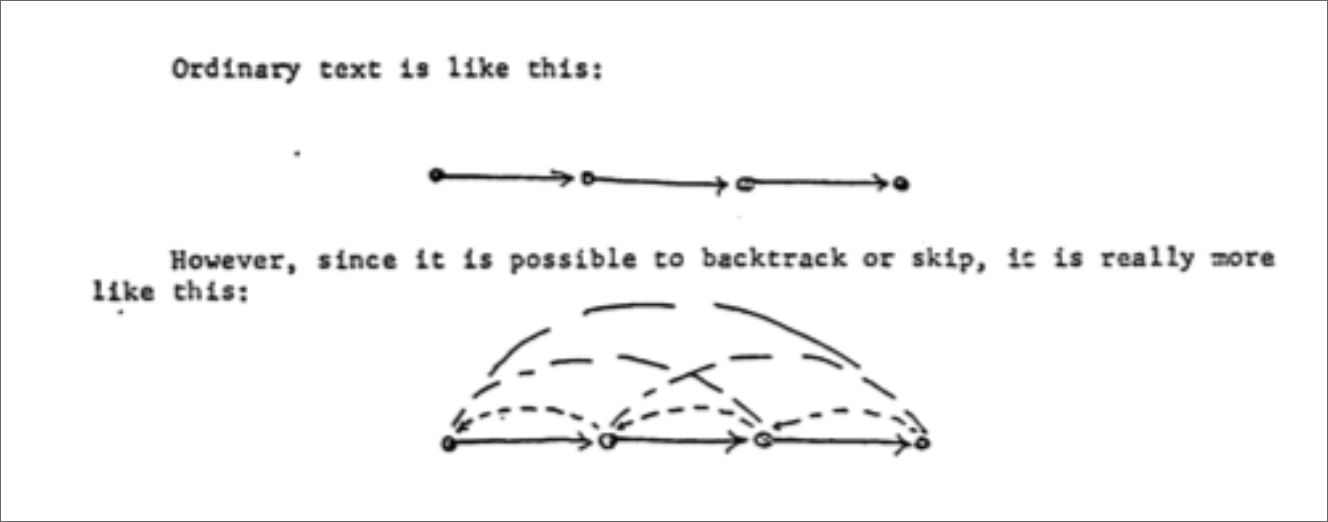
\includegraphics[scale=0.25]{images/H1.png}
    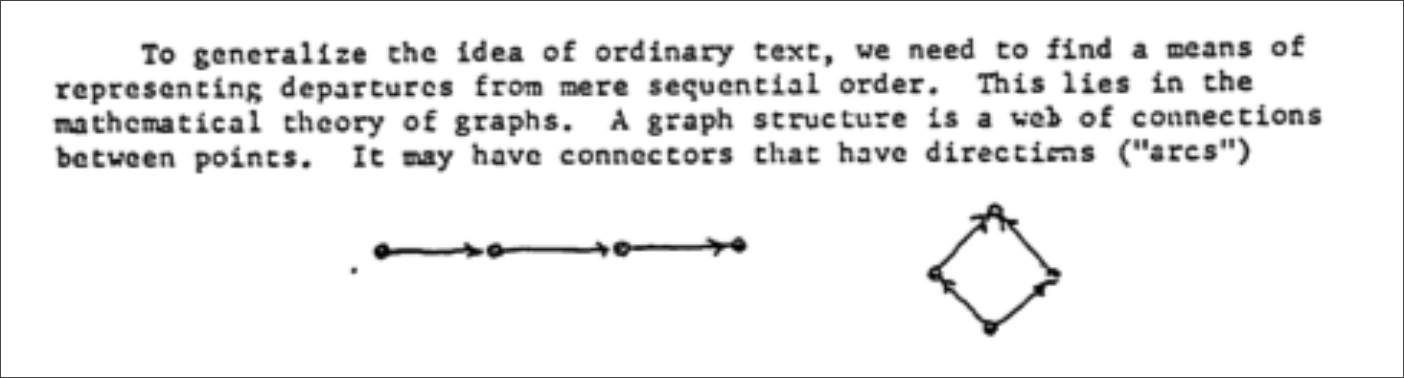
\includegraphics[scale=0.25]{images/H2.png}
    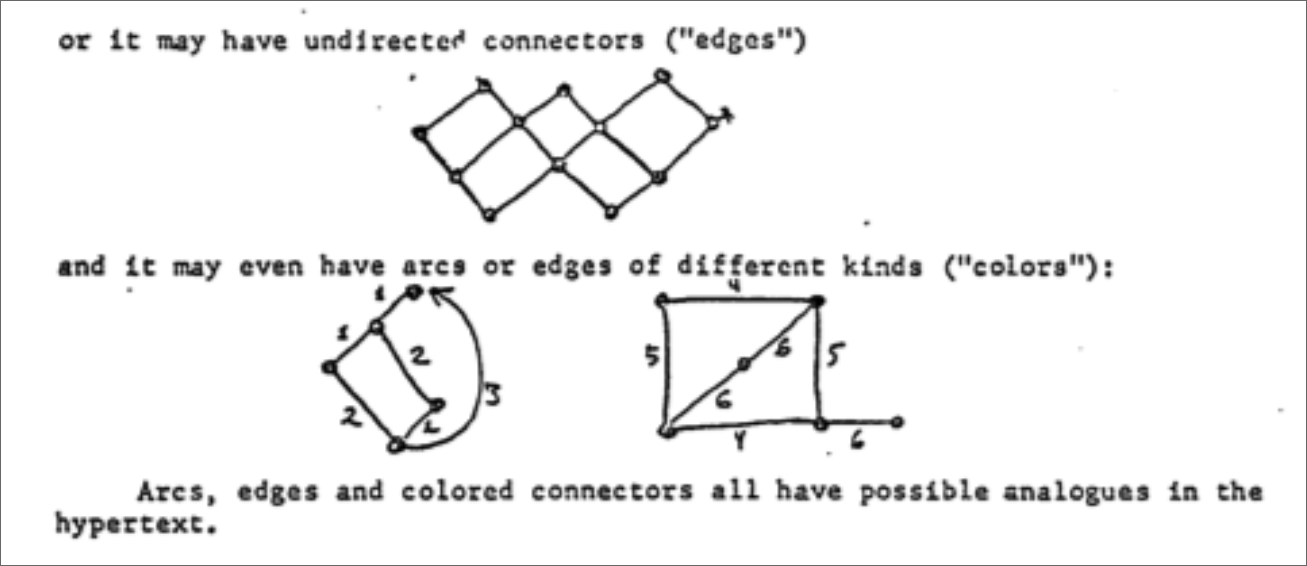
\includegraphics[scale=0.25]{images/H3.png}
\end{figure}

\qs{}{Quali sono i tipi di annotazioni (o connettori) che si possono immaginare in un ipertesto?}

\paragraph{Risposta:}

\begin{itemize}
    \item [$\Rightarrow$] Il \fancyglitter{tag}: un marcatore a cui è allegata una breve nota o spiegazione;
    \item [$\Rightarrow$] Il \fancyglitter{link}: unisce due elementi testuali. È un semplice salto da un punto all'altro.
\end{itemize}

\subsubsection{}

\qs{}{Elencare e descrivere brevemente i tipi di pista (trail) individuati da Nelson nella descrizione del memex di Bush.}

\paragraph{Risposta:}

\begin{itemize}
    \item [$\Rightarrow$] \fancyglitter{Side trails}: piste laterali che si dipartono da una pista principale;
    \item [$\Rightarrow$] \fancyglitter{Skip trails}: sottoinsiemi di una pista principale contenti i punti più importanti.
\end{itemize}

\subsubsection{}

\qs{}{In che senso, come osservato da Nelson, Bush può essere considerato l'origine della nozione di ipertesto?}

\paragraph{Risposta:} Si deve a Bush l'intuizione che la mente umana operi per associazioni.

\qs{}{Fare un esempio di ipertestualità dalla storia delle religioni, indicando esplicitamenti quali aspetti ipertestuali sono coinvolti.}

\begin{itemize}
    \item [$\Rightarrow$] \fancyglitter{Bibbia}: contiene diversi libri che si riferiscono l'uno all'altro;
    \item [$\Rightarrow$] \fancyglitter{Maha\={a}bha\={a}rata}: contiene diversi racconti che si riferiscono l'uno all'altro;
    \item [$\Rightarrow$] \fancyglitter{Talmud}: contiene diversi commenti che si riferiscono l'uno all'altro.
\end{itemize}

\subsubsection{}

\qs{}{Fare un esempio di ipertestualità dalla letteratura scientifica.}

\paragraph{Risposta:} Praticamente ogni articolo scientifico fa riferimento ad altri articoli. Per esempio in ambito matematico 
si fa riferimento a teoremi, dimostrazioni, etc.

\subsubsection{}

\qs{}{Spiegare il concetto di "collaterazione" in Nelson, facendo riferimento alle "zippered lists".}

\paragraph{Risposta:} La collaterazione è un'operazione che permette di creare una lista di elementi che si riferiscono l'uno all'altro, mediante link.
Le zippered lists sono liste che si riferiscono l'una all'altra.

\qs{}{Spiegare brevemente l'idea di "docuverso" in Nelson.}

\paragraph{Risposta:} Un docuverso è un documento che contiene un insieme di documenti che si riferiscono l'uno all'altro.

\subsubsection{}

\qs{}{Spiegare l'idea di "thinkertoy" in Computer Lib/Dream Machines di Nelson, anche commentando i suoi esempi.}

\paragraph{Risposta:} Un thinkertoy è un sistema facile e divertente da usare per aiutare le persone a pensare.
In altre parole è un sistema di visualizzazione
per computer che aiuti a considerare alternative complesse.

\subsubsection{}

\qs{}{Spiegare l'idea di "fantics" (fantica) in Computer Lib/Dream Machines di Nelson, anche commentando i suoi esempi.}

\paragraph{Risposta:} La fantics (fantica) si occupa sia delle arti espressive (scrittura, teatro e così via) sia
delle strutture e dei meccanismi del pensiero.

\begin{itemize}
    \item [$\Rightarrow$] L'arte e la scienza della presentazione;
    \item [$\Rightarrow$] Tecniche di presentazione: scrittura, regia, realizzazione di filmati, etc.
    \item [$\Rightarrow$] I media, la loro analisi, la loro progettazione, etc.;
    \item [$\Rightarrow$] La progettazione di sistemi per le presentazioni.
\end{itemize}

\section{Otlet, Lickider e Kay}

\subsection{Otlet}

\qs{}{Che cosa è il Mundaneum?}

\paragraph{Risposta:} Il Mundaneum è un'organizzazione internazionale fondata da Paul Otlet e Henri La Fontaine.
Dopo la nascita di Internet, il Mundaneum è stato rivalutato come un "Google su carta".

\subsubsection{}

\qs{}{Che cosa è la Mondothèque di Otlet?}

\paragraph{Risposta:} La Mondothèque è un'anticipazione di ciò che diventerà una workstation.

\subsubsection{}

\qs{}{Quali possibilità di trasmissione dei documenti considera Otlet nelle sue visualizzazioni?}

\paragraph{Risposta:} La videoconferenza e la didattica a distanza.

\subsubsection{}

\qs{}{Quali sono i difetti del libro secondo Otlet?}

\paragraph{Risposta:} 

\begin{itemize}
    \item [$\Rightarrow$] Non è pratico per la consultazione di specifici passaggi;
    \item [$\Rightarrow$] È un'entità completa a cui non si può aggiungere nulla;
    \item [$\Rightarrow$] Rende difficile il collegamento di elementi correlati (richiede indicizzazione).
\end{itemize}

\subsubsection{}

\qs{}{Quali sono i vantaggi delle schede realizzate secondo il Principio Monografico?}

\paragraph{Risposta:} L'utilizzo di repertorio, classificazione e ufficio della documentazione.
A ogni scheda del repertorio è associato un solo argomento. Si ha la suddivisione per contenuto informativo.

\subsection{Licklider}

\qs{}{Quali sono gli aspetti comuni tra la concezione del libro di Otlet e quella di Licklider in "Libraries of the Future"?}

\paragraph{Risposta:} Entrambi considerano il libro in veste principalmente negativa,
in quanto non permette di collegare facilmente le informazioni tra loro.

\subsubsection{}

\qs{}{Quale è stato il ruolo di Norbert Wiener nel gruppo cresciuto intorno al Research Laboratory of Electronics del MIT?}

\paragraph{Risposta:} Negli anni '30 Wiener partecipò ai seminari di Arturo Rosenblueth su metodologia e interdisciplinarità
nello studio delle comunicazioni in animali e macchine. Nel 1946 si unisce al gruppo del MIT.
Negli anni successivi partecipò alle Macy Conferences e, organizzava degli incontri il Martedì sera, in cui si 
discuteva di comunicazione come studio dei segnali secondo le leggi generali della teoria dell'informazione di Shannon.

\subsubsection{}

\qs{}{Quali sono i punti deboli nell'utilizzo interattivo del computer, prima del time-sharing?}

\paragraph{Risposta:}

\begin{itemize}
    \item [$\Rightarrow$] Il computer poteva essere utilizzato solo da un utente alla volta;
    \item [$\Rightarrow$] Il sistema precedente era batch processing;
    \item [$\Rightarrow$] Non c'era interazione in tempo reale.
\end{itemize}

\subsubsection{}

\qs{}{Quale può essere una ragionevole divisione dei compiti nella simbiosi uomo-macchina?} 

\paragraph{Risposta:} L'uomo si occupa di problemi complessi, mentre la macchina si occupa di problemi ripetitivi.

\subsubsection{}

\qs{}{Qual è la differenza principale, a livello di linguaggio, tra controllo di una macchina e controllo di un essere umano?}

\paragraph{Risposta:} Gli ordini al computer specificano \fancyglitter{procedure}, mentre gli ordini all'uomo specificano \fancyglitter{obiettivi}.

\subsubsection{}

\qs{}{Fare un esempio di feedback con un insieme di procedure predeterminato che correlano input e output.}

\paragraph{Risposta:} Vedere capitolo \ref{feedback}.

\subsubsection{}

\qs{}{Fare un esempio di feedback (interazione) in assenza di procedure predeterminate che correlano input e output.}

\paragraph{Risposta:} Vedere capitolo \ref{feedback}.

\subsubsection{}

\qs{}{Che cosa era il Memorandum for members and affiliates of the Intergalactic Computer Network di Licklider?}

\paragraph{Risposta:} Era un'idea di una rete geograficamente distribuita di utenti che condividono
risorse di calcolo, file, compilatori e programmi. Può essere considerata l'origine di ARPANET.

\subsubsection{}

\qs{}{Quali sono gli aspetti comuni alla concezione delle biblioteche adottata da Licklider in "Libraries of the Future" e la concezione di Paul Otlet?}

\paragraph{Risposta:} 


\begin{itemize}
    \item [\textcolor{red}{\XSolidBrush}] Schema della biblioteca fisica con scaffali, schede, banchi di consegna, sale di lettura;
    \item [\textcolor{red}{\XSolidBrush}] Schema del libro fisico come archivio passivo di informazione stampata;
    \item [\textcolor{red}{\XSolidBrush}] Schema della pagina stampata come strumento per la memorizzazione a lungo termine;
    \item [\textcolor{green}{\Checkmark}] Gerarchie di segmenti di testo (carattere, parola, frase, paragrafo, capitolo, libro);
    \item [\textcolor{green}{\Checkmark}] La suddivisione in informazione testuale, grafica e figurativa;
    \item [\textcolor{green}{\Checkmark}] Le parti dei documenti (indice, prefazione, appendice, bibliografia, ecc.);
    \item [\textcolor{green}{\Checkmark}] Tipologie di pubblicazioni (libri, riviste, giornali, ecc.);
    \item [\textcolor{green}{\Checkmark}] Infrastrutture come catalogo, indice, etc..
\end{itemize}

\qs{}{Indicare vantaggi e svantaggi della pagine di libro, del libro e della biblioteca}

\begin{figure}[h]
    \centering
    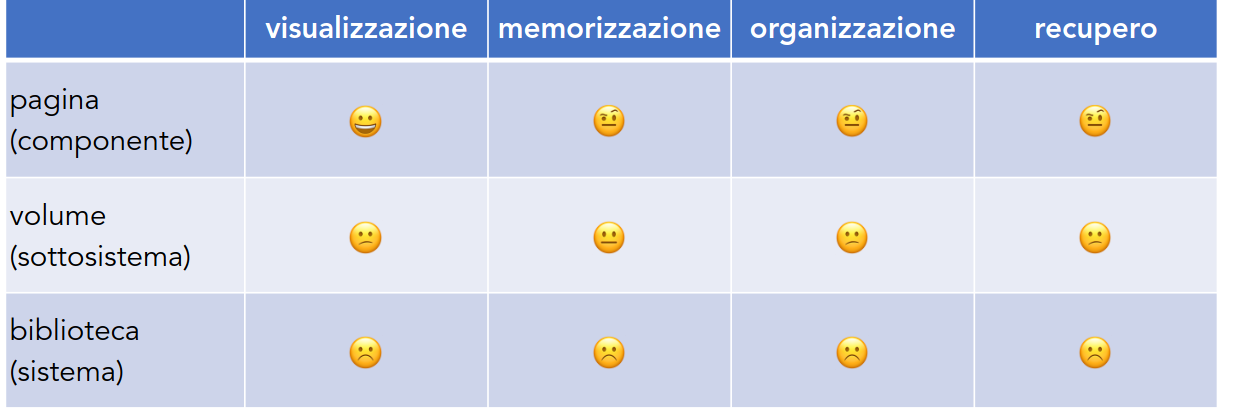
\includegraphics[scale=0.20]{images/Schemi.png}
\end{figure}

\qs{}{In quale senso la pagina stampata è passiva?}

\paragraph{Risposta:} La pagina stampata è passiva perché il trasferimento di informazioni richiede lo spostamento del 
lettore, del libro o di entrambi. Inoltre le operazioni di elaborazione devono essere eseguite dal lettore.

\subsubsection{}

\qs{}{Che cosa è un sistema procognitivo?}

\paragraph{Risposta:} Un sistema procognitivo è una biblioteca del futuro composta da centri di elaborazione dati
connessi tra loro.

\subsection{Alan Kay}

\qs{}{Descrivere sinteticamente il procedimento di condivisione dei file per il computer Burroughs B220 che Alan Kay descrive come primo esempo di astrazione dei dati, nella prospettiva degli oggetti.}

\paragraph{Risposta:} 

\begin{itemize}
    \item [$\Rightarrow$] La prima parte era una \fancyglitter{sequenza di puntatori} alla seconda parte;
    \item [$\Rightarrow$] La seconda parte conteneva le \fancyglitter{procedure} utilizzate per accedere e modificare i dati della terza parte;
    \item [$\Rightarrow$] La terza parte conteneva i \fancyglitter{record} con i dati.
\end{itemize}

\subsubsection{}

\qs{}{In quale modo il funzionamento del sistema Sketchpad di Sutherland può essere confrontato con un linguaggio orientato agli oggetti?}

\paragraph{Risposta:} Kay utilizza una metafora biologica per confrontare Sketchpad con Simula 67:

\begin{itemize}
    \item [$\Rightarrow$] Le cellule ("instances") si conformano ai comportamenti "master";
    \item [$\Rightarrow$] Le cellule sono autonome e comunicano tra loro scambiandosi messaggi;
    \item [$\Rightarrow$] Le cellule diventano parti diverse di un organismo a seconda del contesto.
\end{itemize}

\subsubsection{}

\qs{}{Indicare una metafora-guida nello sviluppo delle idee di Alan Kay sugli oggetti.}

\paragraph{Risposta:} La metafora-guida è quella della biologia.

\subsubsection{}

\qs{}{In quale modo Papert ed il suo linguaggio LOGO hanno influenzato Kay?}

\paragraph{Risposta:} LOGO è un linguaggio di programmazione che permette di creare oggetti grafici.
Papert ha trasmesso a kay l'idea del computer come strumento per l'apprendimento che si 
concretizzò nel progetto Dynabook.

\subsubsection{}

\qs{}{Che cosa si intende dicendo che il computer è un "medium dinamico"?}

\paragraph{Risposta:} Il computer è un medium dinamico perché permette di creare, manipolare e condividere informazioni in modo flessibile.
Non è statico come un libro o un film, ma è interattivo.

\subsubsection{}

\qs{}{In che senso il computer è un medium universale?}

\paragraph{Risposta:} Il computer è un medium universale perché può simulare 
qualsiasi altro medium.
